\documentclass[tikz,border=10pt]{standalone}
\usepackage{tikz}
\usetikzlibrary{shapes.geometric, arrows.meta, positioning, calc, fit, backgrounds}

\begin{document}

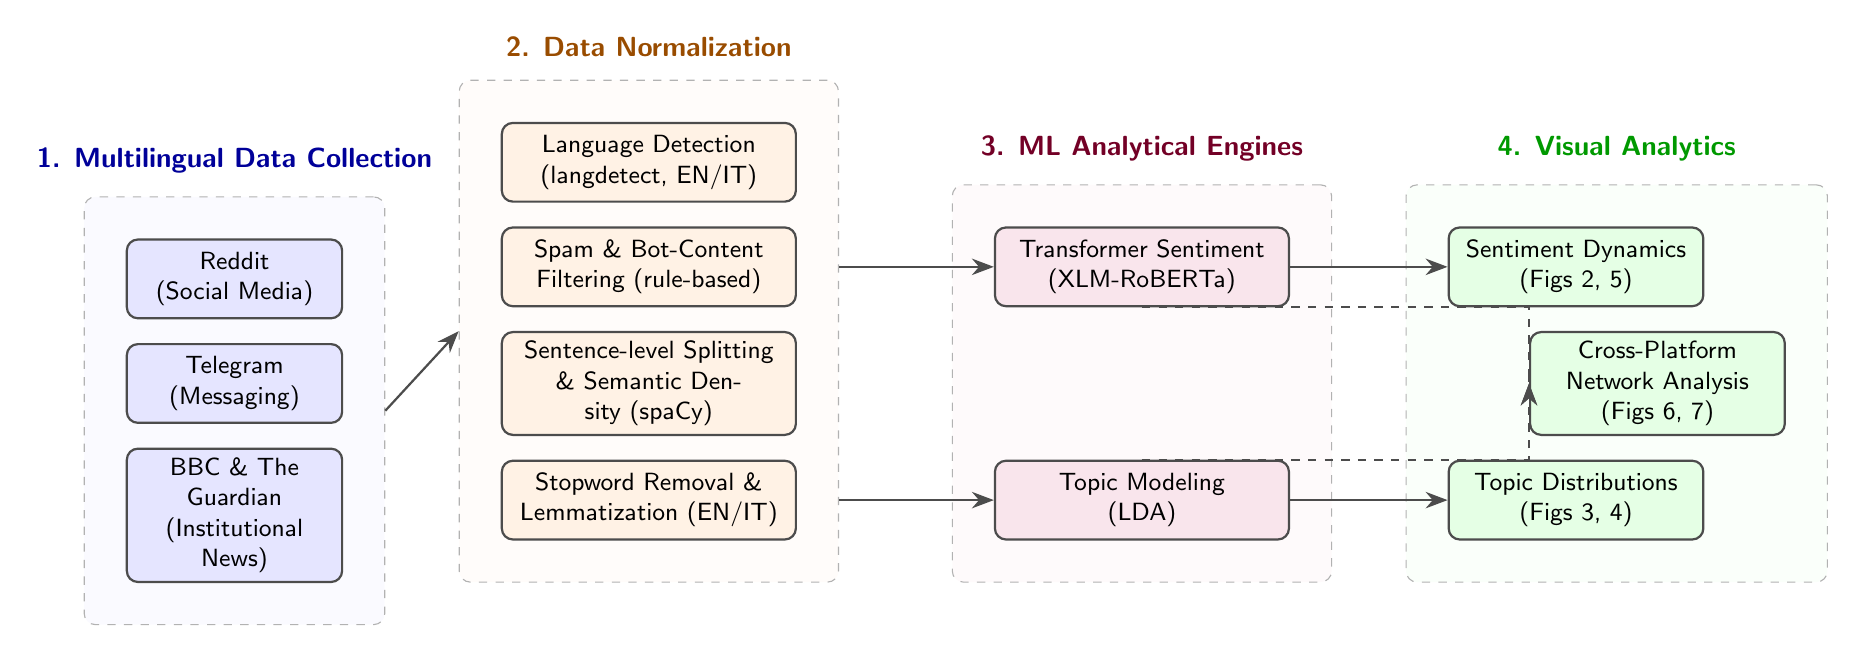
\begin{tikzpicture}[
    auto,
    node distance = 1.5cm and 2.5cm,
    font=\sffamily\small,
    % Styles
    base/.style = {rectangle, rounded corners, draw=black!70, thick, text width=3.5cm, minimum height=1cm, align=center},
    source/.style = {base, fill=blue!10, text width=2.5cm},
    process/.style = {base, fill=orange!10},
    model/.style = {base, fill=purple!10},
    output/.style = {base, fill=green!10, text width=3cm},
    arrow/.style = {-{Stealth[scale=1.2]}, thick, draw=black!70},
    dashed_arrow/.style = {arrow, dashed},
    group_box/.style = {rectangle, rounded corners, draw=black!30, dashed, inner sep=15pt}
]

% --- 1. DATA COLLECTION ---
\node[source] (reddit) {Reddit \\ (Social Media)};
\node[source, below=0.3cm of reddit] (telegram) {Telegram \\ (Messaging)};
\node[source, below=0.3cm of telegram] (news) {BBC \& The Guardian \\ (Institutional News)};

\begin{scope}[on background layer]
    \node[group_box, fill=blue!2, fit=(reddit) (telegram) (news)] (collection_box) {};
    \node[above=5pt of collection_box.north, font=\bfseries\sffamily\color{blue!60!black}] {1. Multilingual Data Collection};
\end{scope}

% --- 2. PREPROCESSING ---
\node[process, right=2cm of telegram] (nlp) {Sentence-level Splitting \\ \& Semantic Density (spaCy)};
\node[process, above=0.3cm of nlp] (split) {Spam \& Bot-Content \\ Filtering (rule-based)};
\node[process, above=0.3cm of split] (langdet) {Language Detection \\ (langdetect, EN/IT)};
\node[process, below=0.3cm of nlp] (lemmatize) {Stopword Removal \& \\ Lemmatization (EN/IT)};

\begin{scope}[on background layer]
    \node[group_box, fill=orange!2, fit=(langdet) (split) (nlp) (lemmatize)] (preproc_box) {};
    \node[above=5pt of preproc_box.north, font=\bfseries\sffamily\color{orange!60!black}] {2. Data Normalization};
\end{scope}

\draw[arrow] (collection_box.east) -- (preproc_box.west);

% --- 3. ANALYTICAL PIPELINE ---
\node[model, right=2.5cm of split] (sentiment) {Transformer Sentiment \\ (XLM-RoBERTa)};
\node[model, right=2.5cm of lemmatize] (topic) {Topic Modeling \\ (LDA)};

\draw[arrow] (preproc_box.east |- sentiment) -- (sentiment);
\draw[arrow] (preproc_box.east |- topic) -- (topic);

\begin{scope}[on background layer]
    \node[group_box, fill=purple!2, fit=(sentiment) (topic)] (model_box) {};
    \node[above=5pt of model_box.north, font=\bfseries\sffamily\color{purple!60!black}] {3. ML Analytical Engines};
\end{scope}

% --- 4. OUTPUT & VISUALIZATION ---
\node[output, right=2cm of sentiment] (out_sent) {Sentiment Dynamics \\ (Figs 2, 5)};
\node[output, right=2cm of topic] (out_topic) {Topic Distributions \\ (Figs 3, 4)};
\node[output, right=2.5cm of model_box] (out_net) {Cross-Platform \\ Network Analysis \\ (Figs 6, 7)};

\draw[arrow] (sentiment) -- (out_sent);
\draw[arrow] (topic) -- (out_topic);
\draw[dashed_arrow] (sentiment.south) -- (out_net.west |- sentiment.south) |- (out_net.west);
\draw[dashed_arrow] (topic.north) -- (out_net.west |- topic.north) |- (out_net.west);

\begin{scope}[on background layer]
    \node[group_box, fill=green!2, fit=(out_sent) (out_topic) (out_net)] (output_box) {};
    \node[above=5pt of output_box.north, font=\bfseries\sffamily\color{green!60!black}] {4. Visual Analytics};
\end{scope}

\end{tikzpicture}
\end{document}
